\documentclass[10pt]{article}
\usepackage[T1]{fontenc}
\usepackage{lmodern}
\usepackage[utf8]{inputenc}
\usepackage{amsmath,amssymb}
\usepackage[a4paper,margin=15mm,top=14mm,bottom=16mm]{geometry}
\usepackage{circuitikz}
\usetikzlibrary{arrows.meta,positioning,calc,decorations.pathreplacing}
\usepackage{array}
\pdftrailerid{}
\raggedright
\setlength{\parindent}{0pt}
\setlength{\parskip}{3pt}
\hyphenpenalty=10000
\exhyphenpenalty=10000
\renewcommand{\arraystretch}{1.15}
% at least 2pt between the boxes of consecutive lines, so linked boxes never touch
\setlength{\normallineskiplimit}{2pt}
\setlength{\normallineskip}{3pt}
\lineskiplimit=\normallineskiplimit
\lineskip=\normallineskip

% ---------------------------------------------------------------------------
% \lk[title]{targets}{content} typesets content and records, at shipout, the
% page and the exact box it occupies, with the Lean it links to, in
% \jobname.lk. guide/make_links.py turns those records into the overlay's
% annotations. Targets are Lean names under the namespace VoltageToBit,
% separated by commas; Name@field is one line of a definition, and
% mod:Path the structural lines of a module.
\makeatletter
\newwrite\lk@out
\immediate\openout\lk@out=\jobname.lk
\newcount\lk@n
\newsavebox\lk@box
\newcommand\lk[3][]{\leavevmode\global\advance\lk@n\@ne
  \sbox\lk@box{#3}%
  \edef\lk@w{\write\lk@out{\the\lk@n|\noexpand\thepage|\noexpand\the\pdflastxpos|%
    \noexpand\the\pdflastypos|\the\wd\lk@box|\the\ht\lk@box|\the\dp\lk@box|\thesection|%
    \detokenize{#1}|\detokenize{#2}}}%
  \pdfsavepos\lk@w\usebox\lk@box}
\makeatother
\newcommand\lkm[3][]{\lk[#1]{#2}{$\displaystyle #3$}}

% notation
\newcommand\psq{\operatorname{psq}}
\newcommand\mlo{\mathrm{lo}}
\newcommand\mhi{\mathrm{hi}}
\newcommand\VDD{V_{\!DD}}
\newcommand\VDDlo{V_{\!DD}^{\mlo}}
\newcommand\VDDhi{V_{\!DD}^{\mhi}}
\newcommand\knlo{k_n^{\mlo}}
\newcommand\knhi{k_n^{\mhi}}
\newcommand\kplo{k_p^{\mlo}}
\newcommand\kphi{k_p^{\mhi}}
\newcommand\Vtnlo{V_{tn}^{\mlo}}
\newcommand\Vtnhi{V_{tn}^{\mhi}}
\newcommand\Vtplo{V_{tp}^{\mlo}}
\newcommand\Vtphi{V_{tp}^{\mhi}}
\newcommand\Clo{C_{\mlo}}
\newcommand\Chi{C_{\mhi}}
\newcommand\VIL{V_{IL}}
\newcommand\VIH{V_{IH}}
\newcommand\VOL{V_{OL}}
\newcommand\VOH{V_{OH}}
\newcommand\Vlo{V_{\mlo}}
\newcommand\Vhi{V_{\mhi}}
\newcommand\uHi{u_{\mathrm{H}}}
\newcommand\uLo{u_{\mathrm{L}}}
\newcommand\Inet{I_{\mathrm{net}}}
\newcommand\Iup{I_{\uparrow}}
\newcommand\Idn{I_{\downarrow}}
\newcommand\RhiP{R^{P}_{\mhi}}
\newcommand\RhiN{R^{N}_{\mhi}}
\newcommand\RloN{R^{N}_{\mlo}}
\newcommand\RloP{R^{P}_{\mlo}}
\newcommand\tup{\tau_{\uparrow}}
\newcommand\tdn{\tau_{\downarrow}}
\newcommand\SafeS{\mathcal S}
\newcommand\Bx{\mathcal B}
\newcommand\rd{\partial^{+}\!}
\newcommand\dec{\operatorname{decode}}
\newcommand\run{\operatorname{Run}}
\newcommand\Hyp{\mathsf{H}}
\newcommand\row{\par\smallskip}
\newcommand\sep{\quad}

\tikzset{
  pm/.style={draw, rounded corners=2pt, inner sep=3pt, font=\footnotesize, align=left},
  ar/.style={-{Stealth[length=5pt]}, thin},
  lab/.style={font=\footnotesize},
}

\begin{document}

{\LARGE\bfseries voltage-to-bit}\hfill{\small CC BY 4.0}\par
\smallskip
{\large One CMOS inverter, from voltages to bits: the specification and its proof}\par
\smallskip
{\small Each framed symbol, formula and node in the viewer opens the Lean lines that state it; between them the links cover every line of the library. Units are volts, microamperes, femtofarads and nanoseconds.}

% ===========================================================================
\section{The circuit}

\begin{minipage}[t]{0.33\linewidth}\vspace{0pt}
\begin{circuitikz}[scale=0.82, transform shape]
  \draw (0,0) node[nmos] (N) {};
  \draw (0,2.3) node[pmos] (P) {};
  \draw (P.D) -- (N.D);
  \draw (P.G) -- (N.G);
  \draw ($(P.G)!0.5!(N.G)$) to[short,*-] ++(-0.8,0) node[left] {$u$};
  \draw (P.S) -- ++(0,0.3) coordinate (top);
  \draw ($(top)+(-0.9,0)$) -- ($(top)+(2.9,0)$);
  \draw (N.S) node[ground] {};
  \coordinate (mid) at ($(P.D)!0.5!(N.D)$);
  \draw (mid) to[short,*-] ++(1.1,0) coordinate (o1) -- ++(2.2,0) coordinate (o2);
  \draw (o1) to[C] ++(0,-1.6) node[ground] {};
  \draw (o2) to[I] ++(0,-1.6) node[ground] {};
  \node[above] at ($(mid)+(0.6,0)$) {$v$};
  \node[above right, lab] at ($(top)+(1.0,0)$) {\lk[supply voltage]{Params.VDD}{$\VDD$}};
  \node[right, lab] at ($(P.east)+(0.05,0.35)$) {\lk[PMOS current]{Ip}{$I_p$}};
  \node[right, lab] at ($(N.east)+(0.05,-0.35)$) {\lk[NMOS current]{In}{$I_n$}};
  \node[lab, align=left] at ($(o1)+(1.05,-0.55)$) {$c\in[$\lk[least capacitance]{Design.Clo}{$\Clo$}$,\,$\lk[largest capacitance]{Design.Chi}{$\Chi$}$]$};
  \node[lab, right] at ($(o2)+(0.35,-0.8)$) {$|w|\le$\,\lk[disturbance bound]{Design.eps}{$\varepsilon$}};
  \node[lab, right] at ($(o2)+(0.35,-0.3)$) {$w$};
\end{circuitikz}
\end{minipage}\hfill
\begin{minipage}[t]{0.64\linewidth}\vspace{2pt}
\lk[a parameter point]{Params}{$\theta$}${}=\bigl($\lk[supply voltage]{Params.VDD}{$\VDD$}$,\ $\lk[NMOS transconductance]{Params.kn}{$k_n$}$,\ $\lk[PMOS transconductance]{Params.kp}{$k_p$}$,\ $\lk[NMOS threshold]{Params.Vtn}{$V_{tn}$}$,\ $\lk[PMOS threshold magnitude]{Params.Vtp}{$V_{tp}$}$\bigr)$
\row
\lkm[positive part squared]{psq}{\psq(x)=\max(x,0)^2}
\row
\lkm[NMOS current]{In}{I_n(\theta,u,v)=\tfrac{k_n}{2}\bigl(\psq(u-V_{tn})-\psq(u-v-V_{tn})\bigr)}
\row
\lkm[PMOS current]{Ip}{I_p(\theta,u,v)=\tfrac{k_p}{2}\bigl(\psq(\VDD-u-V_{tp})-\psq(v-u-V_{tp})\bigr)}
\row
\lkm[net current into the output]{Inet}{\Inet(\theta,u,v)=I_p(\theta,u,v)-I_n(\theta,u,v)}
\row
\begin{tikzpicture}[x=0.55cm,y=0.32cm]
  \draw[->] (-2.4,0) -- (2.6,0) node[right] {\footnotesize$x$};
  \draw[->] (0,-0.3) -- (0,4.3);
  \draw[thick] (-2.2,0) -- (0,0);
  \draw[thick, domain=0:2.0, samples=30] plot (\x,{\x*\x});
  \node[lab, right] at (2.7,2.6) {\lk[psq: case form]{psq_eq_ite}{$\psq x=\begin{cases}x^2&0\le x\\0&\text{else}\end{cases}$}};
\end{tikzpicture}
\end{minipage}

\smallskip
{\footnotesize\textbf{Square law, region by region} (forward: node between ground and supply; reverse: outside)}\par
\smallskip
{\footnotesize
\newcommand\two[2]{$\begin{array}{@{}l@{}}#1\Rightarrow\\ \quad #2\end{array}$}
\begin{tabular}{@{}l@{\ \ }l@{\quad}l@{\quad}l@{}}
 & cutoff & triode & saturation\\
NMOS &
\lk[NMOS cutoff]{In_cutoff}{\two{u\le V_{tn},\ 0\le v}{I_n=0}} &
\lk[NMOS triode]{In_triode}{\two{0\le v\le u-V_{tn}}{I_n=k_n\bigl((u-V_{tn})v-\frac{v^2}{2}\bigr)}} &
\lk[NMOS saturation]{In_sat}{\two{V_{tn}\le u,\ u-V_{tn}\le v}{I_n=\frac{k_n}{2}(u-V_{tn})^2}}\\ \noalign{\vskip 3pt}
PMOS &
\lk[PMOS cutoff]{Ip_cutoff}{\two{\VDD-V_{tp}\le u,\ v\le\VDD}{I_p=0}} &
\lk[PMOS triode]{Ip_triode}{\two{u+V_{tp}\le v\le\VDD}{I_p=k_p\bigl((\VDD-u-V_{tp})(\VDD-v)-\frac{(\VDD-v)^2}{2}\bigr)}} &
\lk[PMOS saturation]{Ip_sat}{\two{u\le\VDD-V_{tp},\ v\le u+V_{tp}}{I_p=\frac{k_p}{2}(\VDD-u-V_{tp})^2}}\\ \noalign{\vskip 3pt}
NMOS rev. &
\lk[NMOS reverse cutoff]{In_rev_cutoff}{\two{v\le0,\ u-v\le V_{tn}}{I_n=0}} &
\lk[NMOS reverse triode]{In_rev_triode}{\two{v\le0,\ V_{tn}\le u}{I_n=-k_n\bigl((u-v-V_{tn})(-v)-\frac{(-v)^2}{2}\bigr)}} &
\lk[NMOS reverse saturation]{In_rev_sat}{\two{u\le V_{tn}\le u-v}{I_n=-\frac{k_n}{2}(u-v-V_{tn})^2}}\\ \noalign{\vskip 3pt}
PMOS rev. &
\lk[PMOS reverse cutoff]{Ip_rev_cutoff}{\two{\VDD\le v,\ v-u\le V_{tp}}{I_p=0}} &
\lk[PMOS reverse triode]{Ip_rev_triode}{\two{\VDD\le v,\ u\le\VDD-V_{tp}}{I_p=-k_p\bigl((v-u-V_{tp})(v-\VDD)-\frac{(v-\VDD)^2}{2}\bigr)}} &
\lk[PMOS reverse saturation]{Ip_rev_sat}{\two{\VDD-V_{tp}\le u,\ u+V_{tp}\le v}{I_p=-\frac{k_p}{2}(v-u-V_{tp})^2}}
\end{tabular}}

\smallskip
{\footnotesize\textbf{Signs and bounds}\quad
\lk[NMOS discharges above ground]{In_nonneg}{$0\le k_n,\ 0\le v\Rightarrow 0\le I_n$}\sep
\lk[NMOS reverse below ground]{In_nonpos}{$0\le k_n,\ v\le0\Rightarrow I_n\le0$}\sep
\lk[PMOS charges below supply]{Ip_nonneg}{$0\le k_p,\ v\le\VDD\Rightarrow 0\le I_p$}\sep
\lk[PMOS reverse above supply]{Ip_nonpos}{$0\le k_p,\ \VDD\le v\Rightarrow I_p\le0$}\par
\lk[NMOS below its saturation current]{In_le_sat}{$0\le k_n\Rightarrow I_n\le\frac{k_n}{2}\psq(u-V_{tn})$}\sep
\lk[PMOS below its saturation current]{Ip_le_sat}{$0\le k_p\Rightarrow I_p\le\frac{k_p}{2}\psq(\VDD-u-V_{tp})$}\sep
\lk[net current is continuous]{continuous_Inet}{$(u,v)\mapsto\Inet(\theta,u,v)$ continuous}\par
\lk[net current is Lipschitz in v]{abs_Inet_sub_le}{$0\le k_n,k_p\Rightarrow|\Inet(\theta,u,v_1)-\Inet(\theta,u,v_2)|\le\bigl(\frac{k_p}{2}(|v_1-u-V_{tp}|+|v_2-u-V_{tp}|)+\frac{k_n}{2}(|u-v_1-V_{tn}|+|u-v_2-V_{tn}|)\bigr)|v_1-v_2|$}\par
\textbf{psq}\quad
\lk{psq_nonneg}{$0\le\psq x$}\sep
\lk{psq_of_nonneg}{$0\le x\Rightarrow\psq x=x^2$}\sep
\lk{psq_of_nonpos}{$x\le0\Rightarrow\psq x=0$}\sep
\lk[psq is monotone]{psq_mono}{$x\le y\Rightarrow\psq x\le\psq y$}\sep
\lk[psq is continuous]{continuous_psq}{$\psq$ continuous}\par
\lk[increments of psq grow]{psq_incr_mono}{$0\le d,\ x\le y\Rightarrow\psq(x{+}d)-\psq x\le\psq(y{+}d)-\psq y$}\sep
\lk[the comparison behind every margin]{psq_sub_le_psq_sub}{$q\le p,\ q\le q',\ p-q\le p'-q'\Rightarrow\psq p-\psq q\le\psq p'-\psq q'$}\par
\lk[psq is locally Lipschitz]{abs_psq_sub_le}{$|\psq x-\psq y|\le(|x|+|y|)\,|x-y|$}}

% ===========================================================================
\section{The design record}

\begin{minipage}[t]{0.6\linewidth}\vspace{0pt}
\lk[design record]{Design}{$D$}\ \ holds 21 numbers:\par
\smallskip
\begin{tabular}{@{}l@{\quad}l@{}}
supply & $[$\lk{Design.VDDlo}{$\VDDlo$}$,\,$\lk{Design.VDDhi}{$\VDDhi$}$]$\\
NMOS, PMOS gain & $[$\lk{Design.knlo}{$\knlo$}$,\,$\lk{Design.knhi}{$\knhi$}$]$\quad $[$\lk{Design.kplo}{$\kplo$}$,\,$\lk{Design.kphi}{$\kphi$}$]$\\
thresholds & $[$\lk{Design.Vtnlo}{$\Vtnlo$}$,\,$\lk{Design.Vtnhi}{$\Vtnhi$}$]$\quad $[$\lk{Design.Vtplo}{$\Vtplo$}$,\,$\lk{Design.Vtphi}{$\Vtphi$}$]$\\
node capacitance & $[$\lk{Design.Clo}{$\Clo$}$,\,$\lk{Design.Chi}{$\Chi$}$]$\\
unmodelled current & $|w|\le$\lk{Design.eps}{$\varepsilon$}\\
input thresholds & \lk{Design.VIL}{$\VIL$}\quad\lk{Design.VIH}{$\VIH$}\\
output thresholds & \lk{Design.VOL}{$\VOL$}\quad\lk{Design.VOH}{$\VOH$}\\
safe range & $[$\lk{Design.Vlo}{$\Vlo$}$,\,$\lk{Design.Vhi}{$\Vhi$}$]$\quad
\lk[the safe range]{Design.Safe}{$\SafeS=[\Vlo,\Vhi]$}\\
input split points & \lk{Design.uHi}{$\uHi$}\quad\lk{Design.uLo}{$\uLo$}
\end{tabular}

\medskip
\lk[the parameter box]{Design.InBox}{$\theta\in\Bx(D)$}\ \ $\iff$\par
\smallskip
\begin{tabular}{@{}lllll@{}}
\lk{Design.InBox.VDD_ge}{$\VDDlo\le\VDD$} & \lk{Design.InBox.kn_ge}{$\knlo\le k_n$} & \lk{Design.InBox.kp_ge}{$\kplo\le k_p$} & \lk{Design.InBox.Vtn_ge}{$\Vtnlo\le V_{tn}$} & \lk{Design.InBox.Vtp_ge}{$\Vtplo\le V_{tp}$}\\
\lk{Design.InBox.VDD_le}{$\VDD\le\VDDhi$} & \lk{Design.InBox.kn_le}{$k_n\le\knhi$} & \lk{Design.InBox.kp_le}{$k_p\le\kphi$} & \lk{Design.InBox.Vtn_le}{$V_{tn}\le\Vtnhi$} & \lk{Design.InBox.Vtp_le}{$V_{tp}\le\Vtphi$}
\end{tabular}

\medskip
\lkm[three-valued decoding]{decode}{\dec(\ell,h,x)=\begin{cases}0&x\le\ell\\1&\text{else if }h\le x\\\bot&\text{else}\end{cases}}
\par
\begin{tabular}{@{}l@{}}\footnotesize
\lk[reading a 0]{decode_eq_false_iff}{$\dec(\ell,h,x)=0\iff x\le\ell$}\\
\footnotesize\lk[reading a 1]{decode_eq_true_iff}{$\ell<h\Rightarrow(\dec(\ell,h,x)=1\iff h\le x)$}\\
\footnotesize\lk[reading no bit]{decode_eq_none_iff}{$\dec(\ell,h,x)=\bot\iff \ell<x<h$}
\end{tabular}
\row
\lk[input decoding]{Design.decodeIn}{$\dec_{\mathrm{in}}=\dec(\VIL,\VIH,\cdot)$}\qquad
\lk[output decoding]{Design.decodeOut}{$\dec_{\mathrm{out}}=\dec(\VOL,\VOH,\cdot)$}
\end{minipage}\hfill
\begin{minipage}[t]{0.37\linewidth}\vspace{0pt}
\begin{tikzpicture}[y=0.6cm, x=0.9cm]
  \draw[->] (0,-0.4) -- (0,9.6) node[above, lab] {volts (not to scale)};
  \foreach \y/\l in {0/\Vlo,1/0,2/\VOL,3/\VIL,5/\VIH,6/\VOH,7/\VDDlo,8/\VDDhi,9/\Vhi}
    {\draw (-0.08,\y) -- (0.08,\y); \node[lab, right] at (0.08,\y) {$\l$};}
  % input bands
  \fill[black!8] (-2.4,-0.4) rectangle (-1.5,3);
  \fill[black!8] (-2.4,5) rectangle (-1.5,9.6);
  \node[lab, rotate=90] at (-2.75,4.6) {input $u$};
  \node[lab] at (-1.95,1.3) {\lk[input reads 0]{Design.decodeIn,decode_eq_false_iff}{$0$}};
  \node[lab] at (-1.95,4) {\lk[input reads no bit]{Design.decodeIn,decode_eq_none_iff}{$\bot$}};
  \node[lab] at (-1.95,7.3) {\lk[input reads 1]{Design.decodeIn,decode_eq_true_iff}{$1$}};
  % output bands
  \fill[black!8] (1.4,-0.4) rectangle (2.3,2);
  \fill[black!8] (1.4,6) rectangle (2.3,9.6);
  \node[lab, rotate=90] at (2.65,4.6) {output $v$};
  \node[lab] at (1.85,0.8) {\lk[output reads 0]{Design.decodeOut,decode_eq_false_iff}{$0$}};
  \node[lab] at (1.85,4) {\lk[output reads no bit]{Design.decodeOut,decode_eq_none_iff}{$\bot$}};
  \node[lab] at (1.85,7.8) {\lk[output reads 1]{Design.decodeOut,decode_eq_true_iff}{$1$}};
  % safe range
  \draw[decorate, decoration={brace, amplitude=4pt}] (3.1,9) -- (3.1,0) node[midway, right=4pt, lab] {\lk[the safe range]{Design.Safe}{$\SafeS$}};
\end{tikzpicture}
\end{minipage}

% ===========================================================================
\section{Runs}

\lk[a run of the circuit]{IsTrajectory}{$v:\mathbb R\to\mathbb R$ is a run of $D$ on $[a,b]$ for an input $u:\mathbb R\to\mathbb R$}\ \ if
\row
\hspace*{1em}\lk[continuity]{IsTrajectory.cont}{(i)\ $v$ is continuous on $[a,b]$,}
\row
\hspace*{1em}\lk[the current balance]{IsTrajectory.incl}{(ii)\ $\begin{array}[t]{@{}l@{}}\forall t\in[a,b)\ \exists v',c:\ v\text{ has right derivative }v'\text{ at }t,\ \ \Clo\le c\le\Chi,\ \text{and}\\ v(t)\in\SafeS\Rightarrow\exists\theta\in\Bx(D):\ |c\,v'-\Inet(\theta,u(t),v(t))|\le\varepsilon.\end{array}$}

\begin{minipage}[t]{0.42\linewidth}\vspace{0pt}
\begin{tikzpicture}[x=0.7cm,y=0.5cm]
  \fill[black!6] (0,0.6) rectangle (8,5.4);
  \draw[dotted] (0,0.6) -- (8,0.6) node[right, lab] {$\Vlo$};
  \draw[dotted] (0,5.4) -- (8,5.4) node[right, lab] {$\Vhi$};
  \draw[thick] plot[smooth] coordinates {(0,1.5) (1.5,1.9) (3,3.1) (4.5,3.8) (6,3.6) (8,4.5)};
  \fill (3,3.1) circle (1.5pt);
  \draw[densely dashed] (3,3.1) -- (4.6,4.6);
  \draw[densely dashed] (3,3.1) -- (4.8,3.6);
  \node[lab, align=left] at (3.4,-0.5) {\lk[(ii) with the canonical right derivative]{IsTrajectory.balance}{$\exists c,\theta:\ c\,\rd v(t)\in\Inet(\theta,u(t),v(t))\pm\varepsilon$}};
  \node[lab] at (5.0,6.2) {\lk[a run has its right derivative]{IsTrajectory.hasDeriv}{$v$ has right derivative $\rd v(t)$ on $[a,b)$}};
\end{tikzpicture}
\end{minipage}\hfill
\begin{minipage}[t]{0.55\linewidth}\vspace{0pt}
\lk[the right derivative as a function]{rderiv}{$\rd v(t)=$ derivative of $v$ at $t$ within $[t,\infty)$}
\row
\lk[restriction]{IsTrajectory.mono}{run on $[a,b]$, $a\le a'$, $b'\le b\Rightarrow$ run on $[a',b']$}
\row
\lk[only the input on the interval matters]{IsTrajectory.congr_input}{run for $u$, $u=u'$ on $[a,b)\Rightarrow$ run for $u'$}
\row
\lk[gluing two runs]{IsTrajectory.concat}{$\begin{array}{@{}l@{}}a\le c\le b,\ v_1\text{ run on }[a,c],\ v_2\text{ run on }[c,b],\ v_1(c)=v_2(c)\\ \Rightarrow\ (t\mapsto t\le c\ ?\ v_1(t):v_2(t))\text{ run on }[a,b]\end{array}$}
\row
{\footnotesize The capacitance $c$ and the point $\theta$ may differ at every instant; outside $\SafeS$ only (i) and a right derivative are required.}
\end{minipage}

% ===========================================================================
\section{The checks}

\lk[admissibility]{Design.Admissible}{$D$ is admissible}\ \ $\iff$ all 26 hold:\par
\smallskip
{\small
\begin{tabular}{@{}l@{\quad}llllll@{}}
ranges & \lk{Design.Admissible.VDD_le}{$\VDDlo\le\VDDhi$} & \lk{Design.Admissible.kn_le}{$\knlo\le\knhi$} & \lk{Design.Admissible.kp_le}{$\kplo\le\kphi$} & \lk{Design.Admissible.Vtn_le}{$\Vtnlo\le\Vtnhi$} & \lk{Design.Admissible.Vtp_le}{$\Vtplo\le\Vtphi$} & \lk{Design.Admissible.C_le}{$\Clo\le\Chi$}\\
positive & \lk{Design.Admissible.VDD_pos}{$0<\VDDlo$} & \lk{Design.Admissible.kn_pos}{$0<\knlo$} & \lk{Design.Admissible.kp_pos}{$0<\kplo$} & \lk{Design.Admissible.C_pos}{$0<\Clo$} & &\\
not negative & \lk{Design.Admissible.Vtn_nonneg}{$0\le\Vtnlo$} & \lk{Design.Admissible.Vtp_nonneg}{$0\le\Vtplo$} & \lk{Design.Admissible.VOL_nonneg}{$0\le\VOL$} & \lk{Design.Admissible.eps_nonneg}{$0\le\varepsilon$} & &\\
safe range & \lk{Design.Admissible.Vlo_le}{$\Vlo\le0$} & \lk{Design.Admissible.Vhi_ge}{$\VDDhi\le\Vhi$} & & & &\\
thresholds & \lk{Design.Admissible.VOL_le_VIL}{$\VOL\le\VIL$} & \lk{Design.Admissible.VIL_lt_VIH}{$\VIL<\VIH$} & \lk{Design.Admissible.VIH_le_VOH}{$\VIH\le\VOH$} & \lk{Design.Admissible.VOH_le}{$\VOH\le\VDDlo$} & &\\
margins & \lk{Design.Admissible.up}{$\varepsilon<\Iup(\VOH)$} & \lk{Design.Admissible.dn}{$\varepsilon<\Idn(\VOL)$} & \lk{Design.Admissible.hiP}{$\varepsilon<\RhiP$} & \lk{Design.Admissible.hiN}{$\varepsilon<\RhiN$} & \lk{Design.Admissible.loN}{$\varepsilon<\RloN$} & \lk{Design.Admissible.loP}{$\varepsilon<\RloP$}
\end{tabular}}

\smallskip
The six margins, worst corners of the box in closed form:\par
\smallskip
\lkm[pull-up margin]{Design.Iup}{\Iup(c)=\tfrac{\kplo}{2}\bigl(\psq(\VDDlo-\VIL-\Vtphi)-\psq(c-\VIL-\Vtphi)\bigr)-\tfrac{\knhi}{2}\psq(\VIL-\Vtnlo)}
\row
\lkm[pull-down margin]{Design.Idn}{\Idn(c)=\tfrac{\knlo}{2}\bigl(\psq(\VIH-\Vtnhi)-\psq(\VIH-c-\Vtnhi)\bigr)-\tfrac{\kphi}{2}\psq(\VDDhi-\VIH-\Vtplo)}
\row
\lkm[restoring current at the top, PMOS]{Design.RhiP}{\RhiP=\tfrac{\kplo}{2}\bigl(\psq(\VDDlo-\uHi-\Vtphi+(\Vhi-\VDDhi))-\psq(\VDDlo-\uHi-\Vtphi)\bigr)}
\sep
\lkm[restoring current at the top, NMOS]{Design.RhiN}{\RhiN=\tfrac{\knlo}{2}\bigl(\psq(\uHi-\Vtnhi)-\psq(\uHi-\Vhi-\Vtnhi)\bigr)}
\row
\lkm[restoring current at the bottom, NMOS]{Design.RloN}{\RloN=\tfrac{\knlo}{2}\bigl(\psq(\uLo-\Vlo-\Vtnhi)-\psq(\uLo-\Vtnhi)\bigr)}
\sep
\lkm[restoring current at the bottom, PMOS]{Design.RloP}{\RloP=\tfrac{\kplo}{2}\bigl(\psq(\VDDlo-\uLo-\Vtphi)-\psq(\Vlo-\uLo-\Vtphi)\bigr)}

% ===========================================================================
\section{Deadlines and the guarantee}

\lkm[rising deadline]{Design.tauUp}{\tup=\frac{\Chi\,(\VOH-\Vlo)}{\Iup(\VOH)-\varepsilon}}
\qquad
\lkm[falling deadline]{Design.tauDn}{\tdn=\frac{\Chi\,(\Vhi-\VOL)}{\Idn(\VOL)-\varepsilon}}
\qquad
\lkm[deadline for an input bit]{Design.tau}{\tau(1)=\tdn,\ \ \tau(0)=\tup}

\smallskip
$\Hyp$:\ \ $D$ admissible, $v$ a run of $D$ on $[a,b]$ for $u$, $v(a)\in\SafeS$, and $a\le s$, $e\le b$. Then
\row
\hspace*{1em}\lk[(S) the output stays safe]{IsTrajectory.safe}{(S)\ \ $v(t)\in\SafeS$ for all $t\in[a,b]$, whatever $u$ does;}
\row
\hspace*{1em}\lk[(R) low in, high out]{IsTrajectory.rise}{(R)\ \ $u\le\VIL$ on $[s,e)\ \Rightarrow\ \VOH\le v(t)$ for $t\in[s,e]$, $t\ge s+\tup$;}
\row
\hspace*{1em}\lk[(F) high in, low out]{IsTrajectory.fall}{(F)\ \ $\VIH\le u$ on $[s,e)\ \Rightarrow\ v(t)\le\VOL$ for $t\in[s,e]$, $t\ge s+\tdn$;}
\row
\hspace*{1em}\lk[(B) the decoded form]{IsTrajectory.decoded}{(B)\ \ $\dec_{\mathrm{in}}(u)=\beta$ on $[s,e)\ \Rightarrow\ \dec_{\mathrm{out}}(v(t))=\lnot\beta$ for $t\in[s,e]$, $t\ge s+\tau(\beta)$.}

\smallskip
\begin{tikzpicture}[x=0.55cm,y=0.5cm]
  \begin{scope}
  \draw[->] (0,0) -- (12.2,0) node[right, lab] {$t$};
  \draw[->] (0,0) -- (0,6.2) node[above, lab] {$v$};
  \foreach \y/\l in {0.6/\Vlo,4.4/\VOH,5.4/\Vhi} {\draw[dotted] (0,\y) -- (11.6,\y); \node[left, lab] at (0,\y) {$\l$};}
  \fill[black!15] (6.2,4.4) rectangle (11,5.4);
  \draw[densely dashed] (1.2,0.6) -- (6.2,4.4);
  \node[lab] at (8.6,4.9) {\lk[(R) the guaranteed region]{IsTrajectory.rise}{$\VOH\le v$}};
  \node[lab, right] at (4.3,1.5) {\lk[the slope while charging]{IsTrajectory.slope_up}{slope $\ge\frac{\Iup(c)-\varepsilon}{\Chi}$}};
  \foreach \x/\l in {1.2/s,11/e} {\draw (\x,-0.12) -- (\x,0.12); \node[below, lab] at (\x,-0.1) {$\l$};}
  \draw (6.2,-0.12) -- (6.2,0.12); \node[below, lab] at (6.2,-0.1) {\lk[rising deadline]{Design.tauUp}{$s+\tup$}};
  \draw[thick] (1.2,-2.1) -- (11,-2.1); \node[lab, below] at (6.1,-2.1) {$u\le\VIL$ on $[s,e)$};
  \end{scope}
  \begin{scope}[xshift=9.4cm]
  \draw[->] (0,0) -- (12.2,0) node[right, lab] {$t$};
  \draw[->] (0,0) -- (0,6.2) node[above, lab] {$v$};
  \foreach \y/\l in {0.6/\Vlo,1.6/\VOL,5.4/\Vhi} {\draw[dotted] (0,\y) -- (11.6,\y); \node[left, lab] at (0,\y) {$\l$};}
  \fill[black!15] (5.2,0.6) rectangle (11,1.6);
  \draw[densely dashed] (1.2,5.4) -- (5.2,1.6);
  \node[lab] at (8.2,1.1) {\lk[(F) the guaranteed region]{IsTrajectory.fall}{$v\le\VOL$}};
  \node[lab, right] at (3.8,4.3) {\lk[the slope while discharging]{IsTrajectory.slope_dn}{slope $\le-\frac{\Idn(c)-\varepsilon}{\Chi}$}};
  \foreach \x/\l in {1.2/s,11/e} {\draw (\x,-0.12) -- (\x,0.12); \node[below, lab] at (\x,-0.1) {$\l$};}
  \draw (5.2,-0.12) -- (5.2,0.12); \node[below, lab] at (5.2,-0.1) {\lk[falling deadline]{Design.tauDn}{$s+\tdn$}};
  \draw[thick] (1.2,-2.1) -- (11,-2.1); \node[lab, below] at (6.1,-2.1) {$\VIH\le u$ on $[s,e)$};
  \end{scope}
\end{tikzpicture}

% ===========================================================================
\section{How the guarantee is proved}

{\footnotesize Margin facts hold for $D$ admissible and every $\theta\in\Bx(D)$; slope facts for runs under $\Hyp$, using (S).}\par
\smallskip
\begin{tikzpicture}[every node/.append style={anchor=west}]
  \newcommand\tl[1]{$\begin{array}{@{}l@{}}#1\end{array}$}
  \node[pm] (hiP) at (0,0) {\lk[top of the range, PMOS branch]{Design.Inet_Vhi_le_neg_RhiP}{$u\le\uHi\Rightarrow\Inet(\theta,u,\Vhi)\le-\RhiP$}};
  \node[pm] (hiN) at (0,-0.85) {\lk[top of the range, NMOS branch]{Design.Inet_Vhi_le_neg_RhiN}{$\uHi\le u\Rightarrow\Inet(\theta,u,\Vhi)\le-\RhiN$}};
  \node[pm] (loN) at (0,-1.9) {\lk[bottom of the range, NMOS branch]{Design.RloN_le_Inet_Vlo}{$\uLo\le u\Rightarrow\RloN\le\Inet(\theta,u,\Vlo)$}};
  \node[pm] (loP) at (0,-2.75) {\lk[bottom of the range, PMOS branch]{Design.RloP_le_Inet_Vlo}{$u\le\uLo\Rightarrow\RloP\le\Inet(\theta,u,\Vlo)$}};
  \node[pm] (vhi) at (5.7,-0.42) {\lk[inwards at the top]{Design.Inet_Vhi_lt}{$\Inet(\theta,u,\Vhi)<-\varepsilon$ for every $u$}};
  \node[pm] (vlo) at (5.7,-2.32) {\lk[inwards at the bottom]{Design.Inet_Vlo_gt}{$\varepsilon<\Inet(\theta,u,\Vlo)$ for every $u$}};
  \node[pm] (bl) at (5.7,-3.55) {\lk[barrier from above]{barrier_le}{\tl{v(a)\le c,\ (v(t)=c\Rightarrow\rd v(t)<0)\\ \Rightarrow v\le c\text{ on }[a,b]}}};
  \node[pm] (bg) at (5.7,-4.75) {\lk[barrier from below]{barrier_ge}{\tl{c\le v(a),\ (v(t)=c\Rightarrow0<\rd v(t))\\ \Rightarrow c\le v\text{ on }[a,b]}}};
  \node[pm, fill=black!8] (S) at (12.0,-2.32) {(S)};
  \draw[ar] (hiP.east) -- (vhi.west); \draw[ar] (hiN.east) -- (vhi.west);
  \draw[ar] (loN.east) -- (vlo.west); \draw[ar] (loP.east) -- (vlo.west);
  \draw[ar] (vhi.east) -- (S.west); \draw[ar] (vlo.east) -- (S.west); \draw[ar] (bl.east) -- (S.west); \draw[ar] (bg.east) -- (S.west);

  \node[pm] (mu) at (0,-6.4) {\lk[pull-up margin holds]{Design.Inet_ge_Iup}{\tl{u\le\VIL,\ v\le c\le\VDDlo\\ \Rightarrow\Iup(c)\le\Inet(\theta,u,v)}}};
  \node[pm] (md) at (0,-7.9) {\lk[pull-down margin holds]{Design.Inet_le_neg_Idn}{\tl{\VIH\le u,\ 0\le c\le v\\ \Rightarrow\Inet(\theta,u,v)\le-\Idn(c)}}};
  \node[pm] (su) at (4.5,-6.4) {\lk[slope while charging]{IsTrajectory.slope_up}{\tl{c\le\VDDlo,\ \varepsilon<\Iup(c),\ u(t)\le\VIL,\ v(t)\le c\\ \Rightarrow\frac{\Iup(c)-\varepsilon}{\Chi}\le\rd v(t)}}};
  \node[pm] (sd) at (4.5,-7.9) {\lk[slope while discharging]{IsTrajectory.slope_dn}{\tl{0\le c,\ \varepsilon<\Idn(c),\ \VIH\le u(t),\ c\le v(t)\\ \Rightarrow\rd v(t)\le-\frac{\Idn(c)-\varepsilon}{\Chi}}}};
  \node[pm] (rb) at (10.75,-6.4) {\lk[rise by a deadline]{rise_by}{\tl{0<m,\ l\le v(a),\ (v\le c\Rightarrow m\le\rd v)\\ \Rightarrow c\le v(t)\text{ for }t\ge a+\frac{c-l}{m}}}};
  \node[pm] (fb) at (10.75,-7.9) {\lk[fall by a deadline]{fall_by}{\tl{0<m,\ v(a)\le h,\ (c\le v\Rightarrow\rd v\le-m)\\ \Rightarrow v(t)\le c\text{ for }t\ge a+\frac{h-c}{m}}}};
  \node[pm, fill=black!8] (R) at (16.65,-6.4) {(R)};
  \node[pm, fill=black!8] (F) at (16.65,-7.9) {(F)};
  \node[pm, fill=black!8] (B) at (16.65,-7.15) {(B)};
  \draw[ar] (mu.east) -- (su.west); \draw[ar] (md.east) -- (sd.west);
  \draw[ar] (su.east) -- (rb.west); \draw[ar] (sd.east) -- (fb.west);
  \draw[ar] (rb.east) -- (R.west); \draw[ar] (fb.east) -- (F.west);
  \draw[ar] (R.south) -- (B.north); \draw[ar] (F.north) -- (B.south);
  \draw[ar] (S.south) -- ++(0,-3.1) -| ($(su.north)+(0.6,0)$);
\end{tikzpicture}

% ===========================================================================
\section{Shorter deadlines from certificates}

\begin{minipage}[t]{0.4\linewidth}\vspace{0pt}
\begin{tikzpicture}[x=0.52cm,y=0.6cm]
  \draw[->] (0,0) -- (9.4,0) node[right, lab] {$t$};
  \draw[->] (0,0) -- (0,4.6) node[above, lab] {$v$};
  \foreach \y/\l in {0.4/{\ell=\Vlo},1.8/c_1,2.8/c_2,3.6/{c_3=\VOH}} {\draw[dotted] (0,\y) -- (9,\y); \node[left, lab] at (0,\y) {$\l$};}
  \draw[thick] (0,0.4) -- (1.2,1.8) -- (3.0,2.8) -- (5.6,3.6);
  \draw[densely dashed] (0,0.4) -- (8.4,3.6);
  \draw (5.6,-0.1) -- (5.6,0.1); \node[below, lab] at (5.6,0) {\lk[time of a list of segments]{riseTime}{$\sum_i\frac{c_i-c_{i-1}}{m_i}$}};
  \draw (8.4,-0.1) -- (8.4,0.1); \node[below, lab] at (8.4,0) {$\tup$};
  \node[lab] at (1.05,0.85) {$m_1$};
  \node[lab] at (2.55,1.75) {$m_2$};
  \node[lab] at (4.9,2.75) {$m_3$};
\end{tikzpicture}
\end{minipage}\hfill
\begin{minipage}[t]{0.58\linewidth}\vspace{0pt}\footnotesize
\lk[time of a rising list]{riseTime}{$\mathrm{riseTime}(\ell,[(c_1,m_1),\dots,(c_k,m_k)])=\sum_i\frac{c_i-c_{i-1}}{m_i},\ c_0=\ell$}\par
\lk[last level of a list]{finalLevel}{$\mathrm{finalLevel}(\ell,[\dots,(c_k,m_k)])=c_k$ ($\ell$ if empty)}\par
\lk[a valid rising list]{RiseSegs}{$\mathrm{RiseSegs}(\ell,\cdot)\iff\ell\le c_1\le\dots\le c_k,\ 0<m_i$}\par
\lk{RiseSegs.pos}{$0<m_i$}\sep\lk{RiseSegs.le_finalLevel}{$\ell\le c_k$}\sep\lk{RiseSegs.mem_le_finalLevel}{$c_i\le c_k$}\sep\lk{riseTime_nonneg}{$0\le\mathrm{riseTime}$}\par
\lk[rise through a list of levels]{rise_chain}{$(v\le c_i\Rightarrow m_i\le\rd v)\ \forall i,\ \ell\le v(s)\Rightarrow c_k\le v(t)$ for $t\ge s+\mathrm{riseTime}$}
\end{minipage}

\smallskip
{\footnotesize
\lk[time of a falling list]{fallTime}{$\mathrm{fallTime}(h,\cdot)=\sum_i\frac{c_{i-1}-c_i}{m_i},\ c_0=h$}\sep
\lk[a valid falling list]{FallSegs}{$\mathrm{FallSegs}(h,\cdot)\iff h\ge c_1\ge\dots\ge c_k,\ 0<m_i$}\sep
\lk{FallSegs.pos}{$0<m_i$}\sep\lk{FallSegs.finalLevel_le}{$c_k\le h$}\sep\lk{FallSegs.finalLevel_le_mem}{$c_k\le c_i$}\sep\lk{fallTime_nonneg}{$0\le\mathrm{fallTime}$}\par
\lk[fall through a list of levels]{fall_chain}{$(c_i\le v\Rightarrow\rd v\le-m_i)\ \forall i,\ v(s)\le h\Rightarrow v(t)\le c_k$ for $t\ge s+\mathrm{fallTime}$}}

\smallskip
\lk[rising slopes from the margin]{Design.upSegs}{$\mathrm{up}(cs)=[(c,\frac{\Iup(c)-\varepsilon}{\Chi}):c\in cs]$}\sep
\lk[falling slopes from the margin]{Design.dnSegs}{$\mathrm{dn}(cs)=[(c,\frac{\Idn(c)-\varepsilon}{\Chi}):c\in cs]$}
\row
\lk[a rising certificate]{Design.ValidRiseCert}{$\mathrm{RiseCert}(cs,\tau)\iff\mathrm{RiseSegs}(\Vlo,\mathrm{up}\,cs)\wedge\mathrm{finalLevel}=\VOH\wedge\mathrm{riseTime}\le\tau$}
\row
\lk[a falling certificate]{Design.ValidFallCert}{$\mathrm{FallCert}(cs,\tau)\iff\mathrm{FallSegs}(\Vhi,\mathrm{dn}\,cs)\wedge\mathrm{finalLevel}=\VOL\wedge\mathrm{fallTime}\le\tau$}
\row
Under $\Hyp$:\ \
\lk[rise through certified levels]{IsTrajectory.rise_certificate}{$\mathrm{RiseSegs}(\Vlo,\mathrm{up}\,cs),\ cs\le\VDDlo,\ u\le\VIL$ on $[s,e)\Rightarrow\mathrm{finalLevel}\le v(t),\ t\ge s+\mathrm{riseTime}$}
\row
\hspace*{3.2em}\lk[fall through certified levels]{IsTrajectory.fall_certificate}{$\mathrm{FallSegs}(\Vhi,\mathrm{dn}\,cs),\ 0\le cs,\ \VIH\le u$ on $[s,e)\Rightarrow v(t)\le\mathrm{finalLevel},\ t\ge s+\mathrm{fallTime}$}
\row
\hspace*{3.2em}\lk[a rising certificate proves its deadline]{IsTrajectory.rise_of_cert}{$\mathrm{RiseCert}(cs,\tau)\Rightarrow$ (R) with $\tau$ for $\tup$}\sep
\lk[a falling certificate proves its deadline]{IsTrajectory.fall_of_cert}{$\mathrm{FallCert}(cs,\tau)\Rightarrow$ (F) with $\tau$ for $\tdn$}

% ===========================================================================
\section{Runs exist and are unique}

$\Hyp_0$:\ \ $D$ admissible, $\theta\in\Bx(D)$, $u,w$ continuous, $|w|\le\varepsilon$ on $[a,b]$, $a\le b$, $v_0\in\SafeS$, $\Clo\le C(x)$ for all $x$, $|C(x)-C(y)|\le K|x-y|$ on $\SafeS$.\par
\smallskip
\begin{tikzpicture}[node distance=3mm]
  \node[pm] (cl) at (0,0) {\lk[clamp]{clamp}{$\mathrm{clamp}(\ell,h,x)=\max(\min(x,h),\ell)$}\\[2pt]
     \lk{clamp_mem}{$\ell\le h\Rightarrow\mathrm{clamp}\in[\ell,h]$}\ \ \lk{clamp_of_mem}{$x\in[\ell,h]\Rightarrow\mathrm{clamp}=x$}\\[2pt]
     \lk[clamp is 1-Lipschitz]{abs_clamp_sub_le}{$|\mathrm{clamp}\,x-\mathrm{clamp}\,y|\le|x-y|$}};
  \node[pm] (cf) at (0,-2.2) {\lk[the clamped right-hand side]{clampedField}{$f(t,x)=\frac{\Inet(\theta,u(t),\bar x)+w(t)}{C(\bar x)},\ \bar x=\mathrm{clamp}(\Vlo,\Vhi,x)$}};
  \node[pm] (bd) at (0,-3.4) {\lk[Lipschitz and bounded]{exists_clampedField_bounds}{$\exists K,L\ge0:\ |f(t,x)-f(t,y)|\le K|x-y|,\ |f(t,x)|\le L$ on $[a,b]$}};
  \node[pm] (ex) at (8.75,-0.4) {\lk[existence]{exists_solution}{$\Hyp_0\Rightarrow\exists v:\ v(a)=v_0,\ v\in\SafeS$ and $C(v)\,v'=\Inet(\theta,u,v)+w$ on $[a,b]$}};
  \node[pm] (od) at (8.75,-1.5) {\lk[solutions are runs]{IsTrajectory.of_ode}{$\theta\in\Bx,\ \Clo\le C\le\Chi,\ |w|\le\varepsilon,\ C(v)\,\rd v=\Inet(\theta,u,v)+w\Rightarrow$ run}};
  \node[pm] (ov) at (8.75,-2.5) {\lk[solutions with drifting parameters are runs]{IsTrajectory.of_ode_varying}{the same with $\theta(t)\in\Bx$ moving in time $\Rightarrow$ run}};
  \node[pm] (et) at (8.75,-3.5) {\lk[runs exist]{exists_trajectory}{$\Hyp_0,\ C\le\Chi\Rightarrow\exists$ run $v$ with $v(a)=v_0$}};
  \node[pm] (ec) at (8.75,-4.5) {\lk[runs exist, constant capacitance]{exists_trajectory_const}{$\Clo\le C\le\Chi$ constant $\Rightarrow\exists$ run $v$, $v(a)=v_0$}};
  \node[pm] (un) at (0,-4.7) {\lk[uniqueness]{solution_unique}{two solutions with $v_1(a)=v_2(a)\in\SafeS$ agree on $[a,b]$}};
  \node[pm] (st) at (4.6,-5.9) {\lk[runs exist for an input with one jump]{exists_trajectory_step}{$u_1,u_2$ continuous, $a\le c\le b\Rightarrow\exists$ run for $(t<c\ ?\ u_1(t):u_2(t))$, $v(a)=v_0$}};
  \draw[ar] (cl) -- (cf); \draw[ar] (cf) -- (bd);
  \draw[ar] (bd.east) -- (ex.west);
  \draw[ar] (ex.south) -- (od.north);
  \draw[ar] (od.east) -- ++(0.4,0) |- (et.east);
  \draw[ar] (et.south) -- (ec.north);
\end{tikzpicture}

% ===========================================================================
\section{Other models of the same node}

\begin{minipage}[t]{0.36\linewidth}\vspace{0pt}
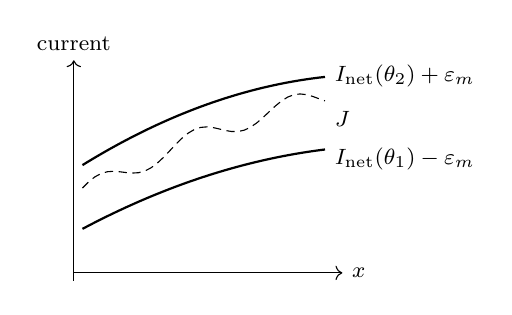
\begin{tikzpicture}[x=0.55cm,y=0.5cm]
  \draw[->] (0,0) -- (6.2,0) node[right, lab] {$x$};
  \draw[->] (0,-0.2) -- (0,5.4) node[above, lab] {current};
  \draw[thick, domain=0.2:5.8, samples=40] plot (\x,{1.0+0.6*\x-0.04*\x*\x});
  \draw[thick, domain=0.2:5.8, samples=40] plot (\x,{2.6+0.7*\x-0.05*\x*\x});
  \draw[densely dashed, domain=0.2:5.8, samples=40] plot (\x,{1.9+0.62*\x-0.03*\x*\x+0.25*sin(160*\x)});
  \node[lab, right] at (5.8,2.9) {$\Inet(\theta_1)-\varepsilon_m$};
  \node[lab, right] at (5.8,5.0) {$\Inet(\theta_2)+\varepsilon_m$};
  \node[lab, right] at (5.8,3.9) {$J$};
\end{tikzpicture}\par
{\footnotesize\lk[a current between two box members]{Design.exists_inBox_of_between}{$\begin{array}{@{}l@{}}\theta_1,\theta_2\in\Bx,\ 0\le\varepsilon,\\ \Inet(\theta_1,u,x)-\varepsilon\le J\le\Inet(\theta_2,u,x)+\varepsilon\end{array}$}\par
\hspace*{1em}\lk[a current between two box members (conclusion)]{Design.exists_inBox_of_between}{$\Rightarrow\exists\theta\in\Bx:\ |J-\Inet(\theta,u,x)|\le\varepsilon$}}
\end{minipage}\hfill
\begin{minipage}[t]{0.61\linewidth}\vspace{0pt}\footnotesize
\lk[mixing two parameter points]{Params.mix}{$\mathrm{mix}(\theta_1,\theta_2,s)=\theta_1+s(\theta_2-\theta_1)$ componentwise}\sep
\lk{Params.mix_zero}{$\mathrm{mix}(\cdot,\cdot,0)=\theta_1$}\sep
\lk{Params.mix_one}{$\mathrm{mix}(\cdot,\cdot,1)=\theta_2$}\par
\lk[current along the mix is continuous]{continuous_Inet_mix}{$s\mapsto\Inet(\mathrm{mix}(\theta_1,\theta_2,s),u,x)$ continuous}\par
\lk[interpolation stays in range]{Design.interp_mem}{$x,y\in[\ell,h],\ s\in[0,1]\Rightarrow x+s(y-x)\in[\ell,h]$}\par
\lk[the box is convex]{Design.InBox.mix}{$\theta_1,\theta_2\in\Bx,\ s\in[0,1]\Rightarrow\mathrm{mix}(\theta_1,\theta_2,s)\in\Bx$}\sep
\lk[NMOS off for low inputs]{Design.InBox.In_eq_zero}{$\theta\in\Bx,\ u\le\Vtnlo,\ 0\le v\Rightarrow I_n=0$}\par
\lk[no current at a grounded node]{Design.InBox.Inet_ground_eq_zero}{$\theta\in\Bx,\ D$ adm., $\VDDhi-\Vtplo\le u\Rightarrow\Inet(\theta,u,0)=0$}\par
\smallskip
\lk[another current law]{IsTrajectory.of_model_error}{$\varepsilon_m+\varepsilon_w\le\varepsilon,\ \forall t,\forall x\in\SafeS\ \exists\theta\in\Bx:|J(t,x)-\Inet(\theta,u(t),x)|\le\varepsilon_m,\ |w|\le\varepsilon_w,$}\par
\hspace*{1em}\lk[another current law (conclusion)]{IsTrajectory.of_model_error}{$v$ continuous, $c\,\rd v=J(t,v)+w$ with $c\in[\Clo,\Chi]\ \Rightarrow$ run}\par
\lk[the sandwich form]{IsTrajectory.of_sandwich}{$0\le\varepsilon_m$, $\Inet(\theta_1,u(t),x)-\varepsilon_m\le J(t,x)\le\Inet(\theta_2,u(t),x)+\varepsilon_m$ on $\SafeS\Rightarrow$ run}\par
\lk[the static sandwich]{IsTrajectory.of_static_sandwich}{$\begin{array}{@{}l@{}}u(t)\in U;\ \forall x\in U,y\in\SafeS:\ \Inet(\theta_1,x,y)-\varepsilon_m\le J(x,y)\le\Inet(\theta_2,x,y)+\varepsilon_m;\\ c\,\rd v=J(u,v)+w\Rightarrow\text{run}\end{array}$}\par
\lk[a slew bound]{slew_bound_of_rderiv}{$u$ continuous, $|\rd u|\le S\Rightarrow|u(t)-u(s)|\le S\,(t-s)$}
\end{minipage}

\smallskip
\begin{minipage}[t]{0.3\linewidth}\vspace{0pt}
\begin{circuitikz}[scale=0.75, transform shape]
  \draw (0,0) node[circ] (n) {} node[above left] {$v$};
  \draw (n) to[C] ++(0,-1.6) node[ground] {};
  \draw (n) to[C] ++(-2.0,0) node[left] {$u$};
  \draw (n) to[C] ++(2.0,0) node[right] {$g$};
  \node[lab] at (0.6,-0.8) {$C_L$};
  \node[lab] at (-1.0,0.75) {$C_M$};
  \node[lab] at (1.0,0.75) {$C_c$};
  \draw (n) -- ++(0,0.8) node[above, lab] {$\Inet(\theta,u,v)+w$};
\end{circuitikz}
\end{minipage}\hfill
\begin{minipage}[t]{0.68\linewidth}\vspace{4pt}\footnotesize
\lk[charge balance with coupling capacitors]{IsTrajectory.of_charge_balance}{$\begin{array}{@{}l@{}}
0\le C_M,C_c,\ \ 0<\Clo\le C_L+C_M+C_c\le\Chi,\ \ C_MS_u+C_cS_g+\varepsilon_w\le\varepsilon,\ \ \theta\in\Bx,\\ |\rd u|\le S_u,\ |\rd g|\le S_g,\ |w|\le\varepsilon_w,\\
q=C_Lv+C_M(v-u)+C_c(v-g)\text{ continuous},\ u,g\text{ continuous},\\ \rd q=\Inet(\theta,u,v)+w\ \Rightarrow\ v\text{ is a run}
\end{array}$}
\end{minipage}

% ===========================================================================
\section{Measured from the actual supply}

\begin{minipage}[t]{0.72\linewidth}\vspace{0pt}\footnotesize
\lk[the record at one supply value]{Design.atSupply}{$D|_{V_0}$: $D$ with $\VDDlo=\VDDhi=V_0$ and $\Vhi=V_0+(\Vhi-\VDDhi)$}\par
\lk[the upper split point is below the PMOS reverse knee]{Design.Admissible.uHi_lt}{$D$ adm.\ $\Rightarrow\uHi<\VDDlo-\Vtphi+(\Vhi-\VDDhi)$}\sep
\lk[the NMOS top margin is unchanged]{Design.Admissible.RhiN_atSupply}{$\VDDlo\le V_0\Rightarrow\RhiN(D|_{V_0})=\RhiN(D)$}\par
\lk[admissible at every supply value]{Design.Admissible.atSupply}{$D$ adm., $V_0\in[\VDDlo,\VDDhi]\Rightarrow D|_{V_0}$ adm.}\sep
\lk[a box point is in its own restricted box]{Design.InBox.atSupply}{$\theta\in\Bx(D)\Rightarrow\theta\in\Bx(D|_{\VDD(\theta)})$}\par
\lk[runs at one supply stay near it]{trajectory_safe_atSupply}{run of $D|_{V_0}$ from $[\Vlo,V_0+(\Vhi-\VDDhi)]$ stays there}\par
\lk[constant-parameter solutions are runs at their supply]{IsTrajectory.of_ode_atSupply}{solution with constant $\theta$ is a run of $D|_{\VDD(\theta)}$}\par
\lk[constant-parameter solutions stay near their supply]{solution_safe_atSupply}{solution with constant $\theta$ from $[\Vlo,\VDD(\theta)+(\Vhi-\VDDhi)]$ stays there}
\end{minipage}\hfill
\begin{minipage}[t]{0.26\linewidth}\vspace{0pt}
\begin{tikzpicture}[y=0.42cm]
  \draw[thick] (0,0) -- (0,6); \node[lab, below] at (0,0) {$\SafeS$};
  \draw[thick] (1.6,0) -- (1.6,4.8); \node[lab, below] at (1.6,0) {at $V_0$};
  \foreach \y/\l in {0/\Vlo,6/\Vhi} \node[lab, left] at (0,\y) {$\l$};
  \node[lab, right] at (1.6,4.8) {$V_0+(\Vhi-\VDDhi)$};
  \draw[dotted] (0,4.0) -- (2.0,4.0) node[right, lab] {$V_0$};
\end{tikzpicture}
\end{minipage}

% ===========================================================================
\section{Speed limits}

\begin{minipage}[t]{0.7\linewidth}\vspace{0pt}\footnotesize
\lk[largest charging current]{Design.IchargeMax}{$I^{\max}_{\uparrow}(u_1,u_2)=\frac{\kphi}{2}\psq(\VDDhi-u_1-\Vtplo)+\frac{\knhi}{2}\psq(u_2-\Vlo-\Vtnlo)$}\sep
\lk{Design.IchargeMax_nonneg}{$0\le I^{\max}_{\uparrow}$}\par
\lk[largest discharging current]{Design.IdischargeMax}{$I^{\max}_{\downarrow}(u_1,u_2)=\frac{\knhi}{2}\psq(u_2-\Vtnlo)+\frac{\kphi}{2}\psq(\Vhi-u_1-\Vtplo)$}\sep
\lk{Design.IdischargeMax_nonneg}{$0\le I^{\max}_{\downarrow}$}\par
\lk[charging current is bounded]{Design.Inet_le_IchargeMax}{$u\in[u_1,u_2],\ \Vlo\le v\Rightarrow\Inet(\theta,u,v)\le I^{\max}_{\uparrow}$}\sep
\lk[discharging current is bounded]{Design.neg_IdischargeMax_le_Inet}{$u\in[u_1,u_2],\ v\le\Vhi\Rightarrow-I^{\max}_{\downarrow}\le\Inet(\theta,u,v)$}\par
Under $\Hyp$ with $u\in[u_1,u_2]$ on $[s,e)$:\par
\lk[the output cannot rise faster]{IsTrajectory.rise_at_most}{$v(s)\le\ell\Rightarrow v(t)\le\ell+\frac{I^{\max}_{\uparrow}+\varepsilon}{\Clo}(t-s)$}\sep
\lk[the output cannot fall faster]{IsTrajectory.fall_at_most}{$\ell\le v(s)\Rightarrow\ell-\frac{I^{\max}_{\downarrow}+\varepsilon}{\Clo}(t-s)\le v(t)$}
\end{minipage}\hfill
\begin{minipage}[t]{0.27\linewidth}\vspace{0pt}
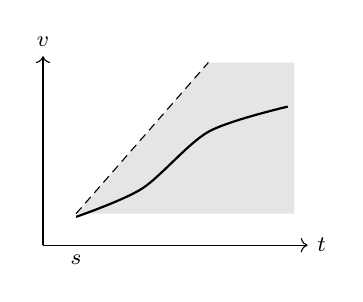
\begin{tikzpicture}[x=0.42cm,y=0.4cm]
  \draw[->] (0,0) -- (8,0) node[right, lab] {$t$};
  \draw[->] (0,0) -- (0,6) node[above, lab] {$v$};
  \fill[black!10] (1,1) -- (5,5.8) -- (7.6,5.8) -- (7.6,1) -- cycle;
  \draw[densely dashed] (1,1) -- (5,5.8);
  \draw[thick] plot[smooth] coordinates {(1,0.9) (3,1.8) (5,3.6) (7.4,4.4)};
  \node[lab, below] at (1,0) {$s$};
\end{tikzpicture}
\end{minipage}

% ===========================================================================
\section{Two inverters in a row}

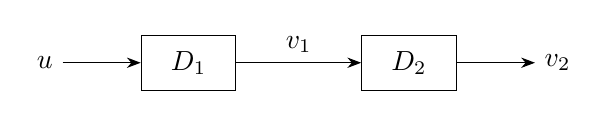
\begin{tikzpicture}[x=1cm]
  \node[draw, minimum width=1.2cm, minimum height=0.7cm] (d1) at (1.6,0) {$D_1$};
  \node[draw, minimum width=1.2cm, minimum height=0.7cm] (d2) at (4.4,0) {$D_2$};
  \draw[ar] (0,0) node[left] {$u$} -- (d1);
  \draw[ar] (d1) -- node[above] {$v_1$} (d2);
  \draw[ar] (d2) -- (6.0,0) node[right] {$v_2$};
\end{tikzpicture}\par
{\footnotesize $v_1$ a run of $D_1$ for $u$, $v_2$ a run of $D_2$ for $v_1$, both admissible, both starting in their safe ranges:}\par
\smallskip
{\footnotesize
\lk[low in, low out of two stages]{chain_low}{$D_2.\VIH\le D_1.\VOH,\ u\le D_1.\VIL$ on $[s,e)\Rightarrow v_2(t)\le D_2.\VOL$ for $t\ge s+D_1.\tup+D_2.\tdn$}\par
\lk[high in, high out of two stages]{chain_high}{$D_1.\VOL\le D_2.\VIL,\ D_1.\VIH\le u$ on $[s,e)\Rightarrow D_2.\VOH\le v_2(t)$ for $t\ge s+D_1.\tdn+D_2.\tup$}\par
\lk[two copies restore a low bit]{chain_restores_low}{$D_1=D_2=D$: $u\le\VIL\Rightarrow v_2\le\VOL$ after $\tup+\tdn$}\sep
\lk[two copies restore a high bit]{chain_restores_high}{$D_1=D_2=D$: $\VIH\le u\Rightarrow\VOH\le v_2$ after $\tdn+\tup$}\par
For the 1.8 V record below:\
\lk[a second stage can be driven]{Examples.exists_second_stage}{$v_1$ continuous on $[0,10]$, $v_0\in[-0.10,2.08]\Rightarrow\exists$ run $v_2$ for $v_1$}\par
\lk[a two-stage run restoring a low bit]{Examples.chain_witness}{$\exists u\le0.40,v_1,v_2$ runs on $[0,10]$, $v_1(0)=v_2(0)=1$: $1.35\le v_1$ on $[3.43,10]$, $v_2\le0.25$ on $[6,10]$}\par
\lk[a two-stage run restoring a high bit]{Examples.chain_witness_high}{$\exists u\ge1.25,v_1,v_2$ runs on $[0,10]$, $v_1(0)=v_2(0)=1$: $v_1\le0.25$ on $[2.57,10]$, $1.35\le v_2$ on $[6,10]$}}

% ===========================================================================
\section{The guarantee is not vacuous}

{\footnotesize For every admissible $D$:\quad
\lk[the box is not empty]{Design.Admissible.exists_inBox}{$\exists\theta\in\Bx(D)$}\sep
\lk{Design.Admissible.VOL_lt_VOH}{$\VOL<\VOH$}\sep
\lk{Design.Admissible.zero_mem_safe}{$0\in\SafeS$}\sep
\lk{Design.Admissible.VOL_mem_safe}{$\VOL\in\SafeS$}\sep
\lk{Design.Admissible.VOH_mem_safe}{$\VOH\in\SafeS$}\sep
\lk{Design.Admissible.tauUp_pos}{$0<\tup$}\sep
\lk{Design.Admissible.tauDn_pos}{$0<\tdn$}\par
\lk[a run that rises]{Design.Admissible.exists_rise_run}{$\exists u\le\VIL$, run $v$ on $[0,\tup+1]$, $v(0)=\VOL$, $\VOH\le v$ on $[\tup,\tup+1]$}\sep
\lk[a run that falls]{Design.Admissible.exists_fall_run}{$\exists u\ge\VIH$, run $v$ on $[0,\tdn+1]$, $v(0)=\VOH$, $v\le\VOL$ on $[\tdn,\tdn+1]$}}

% ===========================================================================
\section{A 1.8 V inverter}

\lk[the illustrative record]{Examples.illustrative}{$D_{1.8}$}\ \ (illustrative, not fitted to any process):\par
\smallskip
{\small
\begin{tabular}{@{}llllll@{}}
\lk{Examples.illustrative@VDDlo}{$\VDDlo=1.62$} & \lk{Examples.illustrative@VDDhi}{$\VDDhi=1.98$} &
\lk{Examples.illustrative@knlo}{$\knlo=160$} & \lk{Examples.illustrative@knhi}{$\knhi=240$} &
\lk{Examples.illustrative@kplo}{$\kplo=80$} & \lk{Examples.illustrative@kphi}{$\kphi=120$}\\
\lk{Examples.illustrative@Vtnlo}{$\Vtnlo=0.45$} & \lk{Examples.illustrative@Vtnhi}{$\Vtnhi=0.60$} &
\lk{Examples.illustrative@Vtplo}{$\Vtplo=0.45$} & \lk{Examples.illustrative@Vtphi}{$\Vtphi=0.60$} &
\lk{Examples.illustrative@Clo}{$\Clo=5$} & \lk{Examples.illustrative@Chi}{$\Chi=20$}\\
\lk{Examples.illustrative@eps}{$\varepsilon=2$} & \lk{Examples.illustrative@VIL}{$\VIL=0.40$} &
\lk{Examples.illustrative@VIH}{$\VIH=1.25$} & \lk{Examples.illustrative@VOL}{$\VOL=0.25$} &
\lk{Examples.illustrative@VOH}{$\VOH=1.35$} & \lk{Examples.illustrative@uHi}{$\uHi=0.77$}\\
\lk{Examples.illustrative@Vlo}{$\Vlo=-0.10$} & \lk{Examples.illustrative@Vhi}{$\Vhi=2.08$} &
\lk{Examples.illustrative@uLo}{$\uLo=0.74$} & & &
\end{tabular}}

\smallskip
\lk[it passes the checks]{Examples.illustrative_admissible}{$D_{1.8}$ admissible}\sep
\lk{Examples.illustrative_eps_pos}{$0<\varepsilon$}\sep
\lk{Examples.illustrative_Iup}{$\Iup(\VOH)=10.476$}\sep
\lk{Examples.illustrative_Idn}{$\Idn(\VOL)=16.296$}\sep
\lk{Examples.illustrative_RhiP}{$\RhiP=2.4$}\sep
\lk{Examples.illustrative_RhiN}{$\RhiN=2.312$}\sep
\lk{Examples.illustrative_RloN}{$\RloN=3.04$}\sep
\lk{Examples.illustrative_RloP}{$\RloP=3.136$}
\row
\lk{Examples.illustrative_tauUp}{$\tup=\frac{7250}{2119}$}\sep
\lk{Examples.illustrative_tauUp_le}{$\tup\le3.43$}\sep
\lk{Examples.illustrative_tauDn}{$\tdn=\frac{4575}{1787}$}\sep
\lk{Examples.illustrative_tauDn_le}{$\tdn\le2.57$}
\row
\lk[the guarantee in numbers]{Examples.illustrative_guarantee}{$\begin{array}{@{}l@{}}v\text{ run of }D_{1.8}\text{ on }[a,b],\ v(a)\in[-0.10,2.08]\ \Rightarrow\ v\in[-0.10,2.08]\text{ on }[a,b],\\
u\le0.40\text{ on }[s,e)\Rightarrow1.35\le v\text{ on }[s+3.43,e],\quad 1.25\le u\text{ on }[s,e)\Rightarrow v\le0.25\text{ on }[s+2.57,e]\end{array}$}
\row
\lk[runs exist for it]{Examples.illustrative_exists}{$\theta\in\Bx,\ C\in[5,20]$ Lipschitz on $[-0.10,2.08]$, $u,w$ continuous, $|w|\le2$, $v_0\in[-0.10,2.08]\Rightarrow\exists$ run, $v(a)=v_0$}\sep
\lk[runs exist, constant capacitance]{Examples.illustrative_exists_const}{the same with $C$ constant}
\row
\lk[runs at one supply stay within 0.10 V of it]{Examples.illustrative_safe_atSupply}{solution with constant $\theta\in\Bx$, $C\in[5,20]$, $|w|\le2$, from $[-0.10,\VDD(\theta)+0.10]$ stays there}

\smallskip
\begin{minipage}[t]{0.47\linewidth}\vspace{0pt}
\begin{tikzpicture}[x=0.68cm,y=0.95cm]
  \draw[->] (0,0) -- (10.6,0) node[right, lab] {$t$};
  \draw[->] (0,0) -- (0,2.3);
  \foreach \x in {0,2,4,6,8,10} {\draw (\x,-0.06) -- (\x,0.06); \node[below, lab] at (\x,0) {$\x$};}
  \draw[thick] (0,1.8) -- (4,1.8) -- (4.2,0) -- (10,0);
  \node[lab, above] at (2,1.8) {$u$};
  \fill[black!15] (2.57,0.08) rectangle (4,0.25);
  \fill[black!15] (7.59,1.35) rectangle (10,2.08);
  \fill (0,1) circle (1.5pt);
  \node[lab, right] at (0.05,1.05) {\lk[it starts undefined]{Examples.illustrative_initial_undefined}{$v(0)=1$ reads $\bot$}};
  \node[lab] at (8.8,2.3) {\lk[an explicit run]{Examples.illustrative_scenario}{$v$ reads 1 on $[7.59,10]$}};
  \node[lab] at (6.7,0.45) {\lk[an explicit run (low part)]{Examples.illustrative_scenario}{$v$ reads 0 on $[2.57,4]$}};
\end{tikzpicture}
{\footnotesize\lk[the ramp input]{Examples.uRamp}{$u(t)=\max(0,\min(1.8,1.8-9(t-4)))$}\par
Only what is proved is drawn: the input, and the windows where the output reads a bit.}
\end{minipage}\hfill
\begin{minipage}[t]{0.5\linewidth}\vspace{0pt}\footnotesize
\lk[nominal parameters]{Examples.nominal}{$\theta_{\mathrm{nom}}=(1.8,200,100,0.5,0.5)$}\sep
\lk{Examples.nominal_inBox}{$\theta_{\mathrm{nom}}\in\Bx$}\par
\lk{Examples.continuous_uRamp}{$u$ continuous}\sep
\lk{Examples.uRamp_high}{$t\le4\Rightarrow u=1.8$}\sep
\lk{Examples.uRamp_low}{$4.16\le t\Rightarrow u\le0.40$}\par
\lk[a sinusoidal disturbance]{Examples.wSin}{$w(t)=2\sin t$}\sep
\lk{Examples.continuous_wSin}{$w$ continuous}\sep
\lk{Examples.abs_wSin_le}{$|w|\le2$}\par
\lk[the explicit run, its equation]{Examples.illustrative_scenario}{$\begin{array}{@{}l@{}}v(0)=1,\ 10\,v'=\Inet(\theta_{\mathrm{nom}},u,v)+w\text{ on }[0,10],\\ v\text{ a run, in }[-0.10,2.08]\end{array}$}\par
\smallskip
\lk[a moving valid-low input]{Examples.uFeed}{$u_f(t)=0.2+0.2\sin10t$}\sep
\lk{Examples.uFeed_le}{$u_f\le0.40$}\sep
\lk{Examples.continuous_uFeed}{$u_f$ continuous}\sep
\lk{Examples.hasDerivAt_uFeed}{$u_f'=2\cos10t$}\par
\lk[an aggressor]{Examples.gFeed}{$g(t)=0.9+0.5\sin10t$}\sep
\lk{Examples.hasDerivAt_gFeed}{$g'=5\cos10t$}\par
\lk[a run with feedthrough and coupling]{Examples.illustrative_feedthrough_scenario}{$\begin{array}{@{}l@{}}\exists v,\ v(0)=1,\ \rd\bigl(9.4v+0.5(v-u_f)+0.1(v-g)\bigr)\\ \quad=\Inet(\theta_{\mathrm{nom}},u_f,v)+0.5\sin t,\ \ v\text{ a run for }u_f,\\ v\text{ reads 1 on }[3.43,10]\end{array}$}
\end{minipage}

% ===========================================================================
\section{How tight the 1.8 V deadlines are}

\begin{tikzpicture}[x=7.0cm]
  \draw[->] (1.45,0) -- (3.68,0) node[right, lab] {rise (ns)};
  \fill[black!22] (1.45,-0.09) rectangle (2.168,0.09);
  \fill[black!6] (2.26,-0.09) rectangle (3.6,0.09);
  \foreach \x in {1.64,2.168,2.26,2.34,3.43} \draw (\x,-0.15) -- (\x,0.15);
  \node[lab, above] at (1.64,0.15) {\lk[false even from 0.25 V]{Examples.rise_deadline_1p64_is_false_from_valid_low}{$1.64$: false from $v(0)=0.25$}};
  \node[lab, above left] at (2.175,0.15) {\lk[false below 2.168]{Examples.rise_deadline_counterexample}{$2.168$}};
  \node[lab, below left] at (2.168,-0.15) {\lk[no certificate below 2.168]{Examples.riseCert_deadline_ge}{every certificate has $\tau\ge2.168$}};
  \node[lab, above right] at (2.253,0.15) {\lk[16 levels prove 2.26]{Examples.illustrative_riseCert_16}{$2.26$ (16 levels)}};
  \node[lab, below right] at (2.30,-0.15) {\lk[3 levels prove 2.34]{Examples.illustrative_riseCert_3}{$2.34$ (3 levels)}};
  \node[lab, below] at (3.05,-0.15) {\lk[the 3-level list does not prove 2.0]{Examples.illustrative_riseCert_rejected}{those 3 levels do not give $2.0$}};
  \node[lab, above] at (3.43,0.15) {closed form $3.43$};
\end{tikzpicture}

\smallskip
\begin{tikzpicture}[x=7.0cm]
  \draw[->] (0.85,0) -- (3.08,0) node[right, lab] {fall (ns)};
  \fill[black!22] (0.85,-0.09) rectangle (1.0234,0.09);
  \fill[black!6] (1.425,-0.09) rectangle (3.0,0.09);
  \foreach \x in {1.0234,1.425,2.57} \draw (\x,-0.15) -- (\x,0.15);
  \node[lab, above] at (1.0234,0.15) {\lk[false below 1.0234]{Examples.fall_deadline_counterexample}{$1.0234$}};
  \node[lab, below] at (1.0234,-0.15) {\lk[no certificate below 1.0234]{Examples.fallCert_deadline_ge}{every certificate has $\tau\ge1.0234$}};
  \node[lab, above] at (1.425,0.15) {\lk[16 levels prove 1.425]{Examples.illustrative_fallCert_16}{$1.425$ (16 levels)}};
  \node[lab, above] at (2.57,0.15) {closed form $2.57$};
\end{tikzpicture}

{\footnotesize Dark: a deadline this short is false. Light: proved. Between them no statement is made.}\par
\smallskip
\lk[the guarantee with 2.26 and 1.425]{Examples.illustrative_guarantee_refined}{the 1.8 V guarantee holds with $2.26$ for $3.43$ and $1.425$ for $2.57$}\par
\lk[rise: false below, true from]{Examples.rise_deadline_bracket}{rise deadline $\tau$: false if $\tau<2.168$, true if $\tau\ge2.26$}\sep
\lk[fall: false below, true from]{Examples.fall_deadline_bracket}{fall deadline $\tau$: false if $\tau<1.0234$, true if $\tau\ge1.425$}
\row
{\footnotesize
\lk[slow pull-up corner]{Examples.slowUpCorner}{$\theta_{\uparrow}=(1.62,240,80,0.60,0.60)$}\sep
\lk{Examples.slowUpCorner_inBox}{$\theta_{\uparrow}\in\Bx$}\sep
\lk{Examples.Inet_slowUp_le}{$-0.10\le x\Rightarrow\Inet(\theta_{\uparrow},0.40,x)\le15.376$}\sep
\lk[below a line]{Examples.le_line_of_rderiv_le}{$\rd v\le m,\ v(a)\le\ell\Rightarrow v(t)\le\ell+m(t-a)$}\par
\lk[a slow rising run]{Examples.slow_rise_run}{$\forall v_0\in\SafeS\ \exists v$: $v(0)=v_0$, $20v'=\Inet(\theta_{\uparrow},0.40,v)-2$, run for $u\equiv0.40$, $v\le v_0+0.6688\,t$}\par
\lk[slow pull-down corner]{Examples.slowDnCorner}{$\theta_{\downarrow}=(1.98,160,120,0.60,0.45)$}\sep
\lk{Examples.slowDnCorner_inBox}{$\theta_{\downarrow}\in\Bx$}\sep
\lk{Examples.Inet_slowDn_ge}{$x\le2.08\Rightarrow-37.76\le\Inet(\theta_{\downarrow},1.25,x)$}\sep
\lk[above a line]{Examples.ge_line_of_rderiv_ge}{$-m\le\rd v,\ h\le v(a)\Rightarrow h-m(t-a)\le v(t)$}\par
\lk[a slow falling run]{Examples.slow_fall_run}{$\forall v_0\in\SafeS\ \exists v$: $v(0)=v_0$, $20v'=\Inet(\theta_{\downarrow},1.25,v)+2$, run for $u\equiv1.25$, $v_0-1.788\,t\le v$}\par
\lk[a larger provable disturbance]{Examples.illustrativeEps}{$D_{1.8}$ with $\varepsilon=2.3801$, $\uHi=0.772486$, $\uLo=0.742506$}\sep
\lk{Examples.illustrativeEps_admissible}{is admissible}\sep
\lk{Examples.illustrativeEps_tauUp}{$\tup=\frac{290000}{80959}$}\sep
\lk{Examples.illustrativeEps_tauDn}{$\tdn=\frac{366000}{139159}$}\par
\lk[no split points help beyond 2.3802]{Examples.illustrative_eps_no_split_points}{$\varepsilon\ge2.3802\Rightarrow D_{1.8}$ with that $\varepsilon$ is inadmissible for every $\uHi,\uLo$}}

% ===========================================================================
\section{Inputs that jump}

\begin{minipage}[t]{0.38\linewidth}\vspace{0pt}
\begin{tikzpicture}[x=0.32cm,y=0.75cm]
  \begin{scope}
  \draw[->] (0,0) -- (11,0) node[right, lab] {$t$};
  \draw[thick] (0,1.8) -- (4,1.8); \draw[thick] (4,0) -- (10,0);
  \fill (4,1.8) circle (2pt); \draw[fill=white] (4,0) circle (2pt);
  \node[lab, below] at (4,0) {$4$};
  \node[lab, above] at (5,1.9) {\lk[old value at the jump]{Examples.uStepL}{$u_L(t)=1.8$ if $t\le4$, else $0$}};
  \end{scope}
  \begin{scope}[yshift=-2.4cm]
  \draw[->] (0,0) -- (11,0) node[right, lab] {$t$};
  \draw[thick] (0,1.8) -- (4,1.8); \draw[thick] (4,0) -- (10,0);
  \draw[fill=white] (4,1.8) circle (2pt); \fill (4,0) circle (2pt);
  \node[lab, below] at (4,0) {$4$};
  \node[lab, above] at (5,1.9) {\lk[new value at the jump]{Examples.uStepR}{$u_R(t)=1.8$ if $t<4$, else $0$}};
  \end{scope}
\end{tikzpicture}
\end{minipage}\hfill
\begin{minipage}[t]{0.6\linewidth}\vspace{0pt}\footnotesize
\lk[they differ only at 4]{Examples.uStepL_eq_uStepR_of_ne}{$t\ne4\Rightarrow u_L(t)=u_R(t)$}\par
\lk[no run for the left-continuous step]{Examples.stepL_no_trajectory}{no run of $D_{1.8}$ for $u_L$ on $[0,10]$ starts in $\SafeS$}\par
\lk[runs for the right-continuous step]{Examples.stepR_has_trajectory}{$\forall v_0\in\SafeS\ \exists$ run for $u_R$ on $[0,10]$, $v(0)=v_0$}\par
\lk[the scope of the guarantee]{Examples.step_input_scope}{both facts at once: the guarantee says nothing for $u_L$ on $[0,10]$}\par
\lk[the ideal step has right derivative 0]{Examples.uStepR_hasDerivWithinAt_zero}{$\rd u_R(t)=0$ for every $t$}\sep
\lk[and is not continuous]{Examples.uStepR_not_continuousOn}{$u_R$ not continuous on $[0,10]$}\par
\lk[a one-instant spike]{Examples.uSpike}{$u_s(t)=1.8$ if $t=0$, else $0$}\sep
\lk[no run through the spike]{Examples.spike_no_trajectory}{no run for $u_s$ on $[0,10]$ with $v(0)\in[-0.02,0.25]$}\par
\lk[the local obstruction]{Examples.no_trajectory_through_left_continuous_jump}{run from $\SafeS$, $u(t_0)=1.8$, $u=0$ on $(t_0,t_0+0.002)$, $v(t_0)\in[-0.02,0.25]\Rightarrow\bot$}\par
\lk[a lower bound on a right derivative]{Examples.rderiv_ge_of_right_nhd}{$\delta>0$, $v$ continuous on $[t_0,t_0+\delta]$, $\rd v\ge m$ on $(t_0,t_0+\delta)\Rightarrow m\le\rd v(t_0)$}\par
\lk[the box in numbers]{Examples.illustrative_box_bounds}{$\theta\in\Bx\Rightarrow\VDD\in[1.62,1.98],\ k_n\in[160,240],\ k_p\in[80,120],\ V_{tn},V_{tp}\in[0.45,0.60]$}\par
\lk{Examples.Inet_high_le}{$x\in[-0.02,0.25]\Rightarrow\Inet(\theta,1.8,x)\le6.6$}\sep
\lk{Examples.Inet_high_ge}{$x\le-0.02\Rightarrow3.8\le\Inet(\theta,1.8,x)$}\sep
\lk{Examples.Inet_low_ge}{$x\in[-0.10,0.45]\Rightarrow41.616\le\Inet(\theta,0,x)$}
\end{minipage}

% ===========================================================================
\section{What breaks it}

{\footnotesize
\begin{tabular}{@{}p{0.2\linewidth}@{\ }p{0.78\linewidth}@{}}
inverted range &
\lk[an inverted NMOS range]{Examples.badBox}{$D_{1.8}$ with $\knlo=300$}\ \
\lk{Examples.badBox_not_admissible}{not admissible}\ \
\lk[its box is empty]{Examples.badBox_empty}{$\Bx=\emptyset$}\\[3pt]
sampling too early &
\lk[no valid high within 38 ps]{Examples.illustrative_no_early_high}{run from $\SafeS$, $u\in[0,0.40]$ on $[s,e)$, $v(s)\le0.25\Rightarrow v(t)<1.35$ for $t\le s+0.038$}\par
\lk[largest rising slew]{Examples.illustrative_max_rise_slew}{$\frac{I^{\max}_{\uparrow}(0,0.40)+\varepsilon}{\Clo}=28.5508$}\ \
\lk[largest falling slew]{Examples.illustrative_max_fall_slew}{$\frac{I^{\max}_{\downarrow}(1.25,1.98)+\varepsilon}{\Clo}=58.3144$}\ \
\lk[38 ps is too early]{Examples.early_sampling_counterexample}{$\exists$ run, $u\le0.40$, $v(0)=0.25$, $v(0.038)<1.35$}\\[3pt]
input below ground &
\lk[fast pull-up corner]{Examples.fastUp}{$\theta_f=(1.98,240,120,0.45,0.45)$}\ \
\lk{Examples.fastUp_inBox}{$\theta_f\in\Bx$}\ \
\lk{Examples.Inet_fastUp_ge}{$x\in[-0.10,1.35]\Rightarrow167.454\le\Inet(\theta_f,-1,x)$}\par
\lk[with u = -1, high within 38 ps]{Examples.valid_low_input_can_give_valid_high_within_38ps}{$u\equiv-1$: $\exists v$, $v(0)=0.25$, $5v'=\Inet(\theta_f,-1,v)$, a run, $1.35\le v(0.038)$}\\[3pt]
no slew bound &
\lk[rising slew unbounded]{Examples.valid_low_rise_slew_unbounded}{$\forall M\ \exists$ run, $u\le0.40$, $v(0)=0.25$, $\rd v(0)>M$}\ \
\lk[falling slew unbounded]{Examples.valid_high_fall_slew_unbounded}{$\forall M\ \exists$ run, $u\ge1.25$, $v(0)=1.35$, $\rd v(0)<-M$}\\[3pt]
swapped transistors &
\lk[the miswired network]{Examples.InetSwapped}{$I^{\times}(\theta,u,v)=\frac{k_n}{2}\bigl(\psq(u-v-V_{tn})-\psq(u-\VDD-V_{tn})\bigr)-\frac{k_p}{2}\bigl(\psq(v-u-V_{tp})-\psq(0-u-V_{tp})\bigr)$}\par
\lk{Examples.InetSwapped_le}{$u\le0.40,\ 1.2\le L\Rightarrow I^{\times}(\theta_{\mathrm{nom}},u,L)\le-50(L-0.9)^2$}\par
\lk[it never goes high]{Examples.miswired_never_high}{$|c\,\rd v-I^{\times}(\theta_{\mathrm{nom}},u,v)|\le2$, $c\in[5,20]$, $u\le0.40$, $v(a)<1.35\Rightarrow v<1.35$ on $[a,b]$}\par
\lk[a run that never goes high]{Examples.miswired_counterexample}{$\forall T\ \exists u\le0.40$, $v(0)\in[-0.10,2.08]$, $v$ in that inclusion on $[0,T]$, $v<1.35$ always}\\[3pt]
too much noise &
\lk[a noisy record]{Examples.noisy}{$D_{1.8}$ with $\varepsilon=10.76$}\ \
\lk{Examples.noisy_not_admissible}{not admissible}\ \
\lk[weak pull-up corner]{Examples.weakCorner}{$\theta_w=(1.62,240,80,0.45,0.60)$}\ \
\lk{Examples.weakCorner_inBox}{$\theta_w\in\Bx$}\par
\lk[the guarantee is then false]{Examples.noisy_counterexample}{$\forall T\ \exists u\le\VIL$, run on $[0,T]$ from $\SafeS$ with $v<\VOH$ always}
\end{tabular}}

% ===========================================================================
\section{Where it is in the code}

{\footnotesize Each node opens a module's imports, its header comment and the lines between its declarations.}\par
\smallskip
\begin{tikzpicture}[mod/.style={draw, rounded corners=2pt, font=\footnotesize, inner sep=2pt}]
  \node[font=\footnotesize\bfseries] at (0,0.7) {\lk[the library root]{mod:VoltageToBit}{VoltageToBit}};
  \node[font=\footnotesize\itshape] at (-6.5,0) {Model};
  \node[font=\footnotesize\itshape] at (-1.5,0) {Proofs};
  \node[font=\footnotesize\itshape] at (4.5,0) {Examples};
  \node[mod] at (-6.5,-0.7) {\lk{mod:Model/PosSq}{PosSq}};
  \node[mod] at (-6.5,-1.4) {\lk{mod:Model/Device}{Device}};
  \node[mod] at (-6.5,-2.1) {\lk{mod:Model/Inverter}{Inverter}};
  \node[mod] at (-3.2,-0.7) {\lk{mod:Proofs/Margins}{Margins}};
  \node[mod] at (-3.2,-1.4) {\lk{mod:Proofs/Reach}{Reach}};
  \node[mod] at (-3.2,-2.1) {\lk{mod:Proofs/Guarantee}{Guarantee}};
  \node[mod] at (-3.2,-2.8) {\lk{mod:Proofs/Certificate}{Certificate}};
  \node[mod] at (-3.2,-3.5) {\lk{mod:Proofs/NonVacuity}{NonVacuity}};
  \node[mod] at (-0.4,-0.7) {\lk{mod:Proofs/Existence}{Existence}};
  \node[mod] at (-0.4,-1.4) {\lk{mod:Proofs/Concat}{Concat}};
  \node[mod] at (-0.4,-2.1) {\lk{mod:Proofs/ModelError}{ModelError}};
  \node[mod] at (-0.4,-2.8) {\lk{mod:Proofs/AtSupply}{AtSupply}};
  \node[mod] at (-0.4,-3.5) {\lk{mod:Proofs/Contamination}{Contamination}};
  \node[mod] at (-0.4,-4.2) {\lk{mod:Proofs/Chain}{Chain}};
  \node[mod] at (3.0,-0.7) {\lk{mod:Examples/IllustrativeDesign}{IllustrativeDesign}};
  \node[mod] at (3.0,-1.4) {\lk{mod:Examples/Illustrative}{Illustrative}};
  \node[mod] at (3.0,-2.1) {\lk{mod:Examples/RefinedDeadlines}{RefinedDeadlines}};
  \node[mod] at (3.0,-2.8) {\lk{mod:Examples/DeadlineBrackets}{DeadlineBrackets}};
  \node[mod] at (6.4,-0.7) {\lk{mod:Examples/Limits}{Limits}};
  \node[mod] at (6.4,-1.4) {\lk{mod:Examples/InputClass}{InputClass}};
  \node[mod] at (6.4,-2.1) {\lk{mod:Examples/TwoStage}{TwoStage}};
  \node[mod] at (6.4,-2.8) {\lk{mod:Examples/NegativeControls}{NegativeControls}};
\end{tikzpicture}

\end{document}
